\documentclass{beamer}
\usetheme{metropolis}

\usepackage[ngerman]{babel}
\usepackage[autostyle=true,german=quotes]{csquotes}
\usepackage[linewidth=1pt]{mdframed}
\usepackage{hyperref}
\usepackage{makecell}
\usepackage{pifont}
\usepackage{tikz}
\usetikzlibrary{positioning, calc, arrows, fit, decorations.pathreplacing, shapes, shapes.multipart, snakes}
\usepackage{verbatim}
\usepackage{textcomp}
\usepackage{centernot}
\usepackage{tabularx}
\usepackage{ulem}
%\usepackage{pdfpages}

\batchmode

\hypersetup{
	colorlinks,
	urlcolor=blue,
	linkcolor=black % for ToC
}
\newenvironment{qaa}[1]{
	#1

	\begin{mdframed}
		\small
}{
	\end{mdframed}
}

\newcommand{\true}{\ding{51}}
\newcommand{\false}{\ding{55}}
\newcommand{\code}[1]{
	\begin{mdframed}
		\verbatiminput{#1}
	\end{mdframed}
}


\title{Tutorium 11: Typinferenz}
% \subtitle{}
\author{Paul Brinkmeier}
\institute{Tutorium Programmierparadigmen am KIT}
\date{02. Februar 2021}

\begin{document}

\begin{frame}
	\titlepage
\end{frame}

\section{Heutiges Programm}

\begin{frame}{Programm}
	\begin{itemize}
		\item Unifikation
                \begin{itemize}
                  \item Robinson-Algorithmus
                  \item Allgemeinster Unifikator (mgu)
                \end{itemize}
		\item Typinferenz
                \begin{itemize}
                  \item Regelsystem mit Ableitungsbäumen
                  \item Constraint-System
                  \item Unifikation zu einem mgu
                \end{itemize}
	\end{itemize}
\end{frame}

\section{Unifikation}

\subsection{Problemstellung}

\begin{frame}{Welche Probleme löst die Unifikation?}
  \begin{align*}
    \functor{state}{\pa{l}, \pa{l}, \pa{l}, \pa{l}} &\plsunify \functor{state}{M, W, Z, K} \\
    \functor{opposite}{M, M_2}                       &\plsunify \functor{opposite}{\pa{l}, \pa{r}} \\
    Z                                               &\plsunify K \\
  \end{align*}

  \only<1>{
    \begin{itemize}
      \item Unifikation löst Gleichungssysteme von baumförmigen Termen (hier: Prolog-Terme).
      \item Eingabe: Menge $C = \{ \theta_l^1 \plsunify \theta_r^1, ..., \theta_l^n \plsunify \theta_r^n \}$
      \begin{itemize}
        \item Alle $\theta_{\{l, r\}}^i$ sind Bäume und können Variablen enthalten.
      \end{itemize}
      \item Ausgabe: \emph{Unifikator} $\sigma$, sodass $\sigma(\theta_l^i) = \sigma(\theta_r^i)$.
      \begin{itemize}
        \item Wenn $C$ nicht unifizierbar (bspw. $X = \functor{f}{X}$): \texttt{fail}
      \end{itemize}
    \end{itemize}
  }

  \only<2>{
    Mehrere mögliche Lösungen:

    \begin{align*}
      \sigma_1 &=
        \unifier{\su{M_2}{\pa{r}}} \circ
        \unifier{\su{K}{\pa{l}}} \circ
        \unifier{\su{Z}{\pa{l}}} \circ
        \unifier{\su{W}{\pa{l}}} \circ
        \unifier{\su{M}{\pa{l}}} \\
      \sigma_2 &=
        \unifier{\su{M_2}{\pa{r}}} \circ
        \unifier{\su{K}{\pa{l}}} \circ
        \unifier{\su{Z}{\pa{K}}} \circ
        \unifier{\su{W}{\pa{l}}} \circ
        \unifier{\su{M}{\pa{l}}}
    \end{align*}

    \begin{itemize}
      \item I.d.R. suchen wir nach \emph{einem} allgemeinsten Unifikator (mgu).
      \item mgu $\approx$ minimaler Unifikator, der $C$ löst.
    \end{itemize}
  }
\end{frame}

\subsection{Robinson-Algorithmus}

{
\setbeamercolor{background canvas}{bg=}
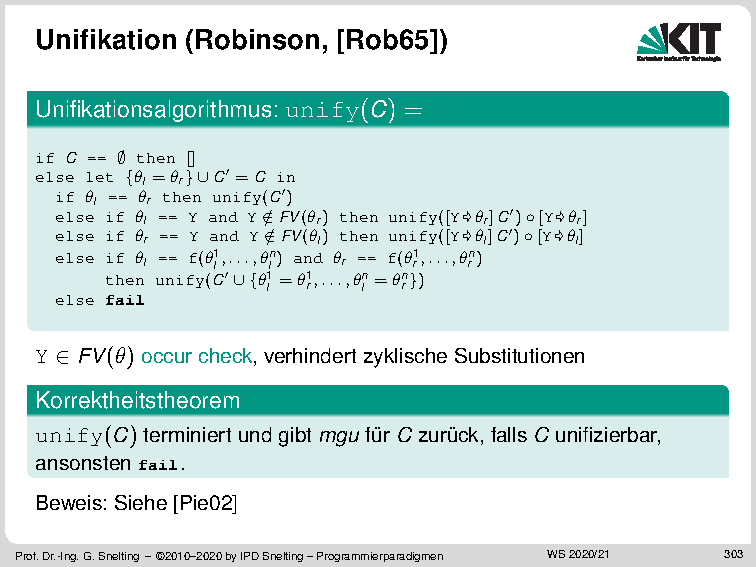
\includepdf{robinson.pdf}
}

\begin{frame}{Robinson-Algorithmus: Zeile für Zeile}
  \only<1>{
    \begin{align*}
      &\texttt{if} \;\; C == \emptyset \;\; \texttt{then} \;\; [] \\
      &\texttt{else let} \;\; \{ \theta_l \plsunify \theta_r \} \cup C' = C \;\; \texttt{in}
    \end{align*}

    \begin{itemize}
      \item Ist das Gleichungssystem $C$ leer, ist es schon gelöst \\
            $\leadsto$ wir brauchen nichts zu ersetzen.
      \item Andernfalls betrachten wir \emph{eine} der Gleichungen: $\theta_l \plsunify \theta_r$.
      \begin{itemize}
        \item \emph{Beliebige Auswahl möglich}.
        \item Die restlichen Gleichungen merken wir uns als $C'$.
      \end{itemize}
    \item Beispiel:\\
          $C = \{ X \plsunify \pa{a}, Y \plsunify \functor{f}{X}, \functor{f}{Z} \plsunify Y \}$\\
          $\theta_l = X, \theta_r = \pa{a}, C' = \{ Y \plsunify \functor{f}{X}, \functor{f}{Z} \plsunify Y \}$
    \end{itemize}
  }

  \only<2>{
    \begin{align*}
      &\texttt{if} \;\; \theta_l == \theta_r \;\; \texttt{then unify}(C')
    \end{align*}

    \begin{itemize}
      \item Wenn die Gleichung trivial ist (auf beiden Seiten steht schon das gleiche), brauchen wir auch nichts zu ersetzen.
      \item Wir müssen also nur $C'$ unifizieren.
      \item Verschiedene Gleichheitsrelationen:
      \begin{itemize}
        \item $A \plsunify B$: Element von $C$, behandeln wir wie eine Datenstruktur.
        \item $A == B$: Vergleichsoperator
        \item $A = B$: Meta-Gleichheitsoperator, Notation für Pattern-Matching
      \end{itemize}
    \end{itemize}
  }

  \only<3>{
    \begin{align*}
      &\texttt{else if} \;\; \theta_l == Y \;\; \texttt{and} \;\; Y \not\in FV(\theta_r) \;\; \\
      &\; \texttt{then unify}(\unifier{\su{Y}{\theta_r}} C') \circ \unifier{\su{Y}{\theta_r}} \\
    \end{align*}

    \begin{itemize}
      \item Steht auf der linken Seite eine Variable, so wird diese ersetzt.
      \begin{itemize}
        \item $\theta_l == Y$: \enquote{Ist der Term $\theta_l$ eine Variable $Y$?}
        \item $Y \not\in FV(\theta_r)$: \emph{occurs check}, $Y$ darf sich nicht selbst einsetzen.
      \end{itemize}
      \item Wir ersetzen in $C'$ dann $Y$ durch $\theta_r$.
      \item Substitution $\unifier{\su{Y}{\theta_r}}$ wird als Ergebnis vorgemerkt.
      \item Beispiel: $\theta_l = X$ \true, $X \not\in FV(\theta_r) = FV(\pa{a}) = \emptyset$ \true, d.h.\\
            Ergebnis: $\texttt{unify}(\{ Y \plsunify \functor{f}{\pa{a}}, \functor{f}{Z} \plsunify Y \}) \circ \unifier{\su{A}{\pa{a}}}$
    \end{itemize}
  }

  \only<4>{
    \begin{align*}
      &\texttt{else if} \;\; \theta_r == Y \;\; \texttt{and} \;\; Y \not\in FV(\theta_l) \;\; \\
      &\; \texttt{then unify}(\unifier{\su{Y}{\theta_l}} C') \circ \unifier{\su{Y}{\theta_l}} \\
    \end{align*}

    \begin{itemize}
      \item Auch wenn rechts eine Variable steht muss sie ersetzt werden.
      \item Beispiel: $\theta_r = Y$ \true, $X \not\in FV(\theta_l) = FV(\functor{f}{Z}) = \{ Z \}$ \true, d.h.\\
        Ergebnis: $\texttt{unify}(\{ \functor{f}{Z} \plsunify \functor{f}{\pa{a}} \}) \circ \unifier{\su{Y}{f(Z)}}$
    \end{itemize}
  }

  \only<5>{
    \begin{align*}
      &\texttt{else if} \;\; \theta_l == \functor{f}{\theta_l^1, ..., \theta_r^n} \;\; \texttt{and} \;\; \theta_r == \functor{f}{\theta_r^1, ..., \theta_r^n} \\
      &\; \texttt{then unify}(C' \cup \{ \theta_l^1 \plsunify \theta_r^1, ..., \theta_l^n \plsunify \theta_r^n \})
    \end{align*}

    \begin{itemize}
      \item Steht auf beiden Seiten ein Funktor, extrahieren wir paarweise neue Gleichungen und unifizieren diese mitsamt $C'$.
      \begin{itemize}
        \item Namen der Funktoren \emph{müssen identisch sein}! (hier: \texttt{f})
        \item Parameterzahlen der Funktoren \emph{müssen identisch sein}!
        \item Für Atome: $n = 0$, aber schon abgedeckt durch den ersten Fall.
      \end{itemize}
    \item Beispiel: $\theta_l = \functor{f}{Z}, \theta_r = \functor{f}{\pa{a}}$ \true, $C' = \emptyset$\\
          Ergebnis: $\texttt{unify}(\emptyset \cup \{ Z \plsunify \pa{a} \}) = \unifier{\su{Z}{\pa{a}}}$ (links Variable)
    \end{itemize}
  }
\end{frame}

\begin{frame}{Eine vollständige Ausführung}
  \begin{equation*}
    C = \{ X \plsunify \pa{a}, Y \plsunify \functor{f}{X}, \functor{f}{Z} \plsunify Y \}
  \end{equation*}

  \begin{align*}
    \texttt{unify}(C)
    &= \texttt{unify}(\{ \underline{X \plsunify \pa{a}}, Y \plsunify \functor{f}{X}, \functor{f}{Z} \plsunify Y \}) \\
    &= \texttt{unify}(\{ Y \plsunify \functor{f}{\pa{a}}, \underline{\functor{f}{Z} \plsunify Y} \}) \circ \unifier{\su{X}{\pa{a}}} \\
    &= \texttt{unify}(\{ \underline{\functor{f}{Z} \plsunify \functor{f}{\pa{a}}} \}) \circ \unifier{\su{Y}{\functor{f}{Z}}} \circ \unifier{\su{X}{\pa{a}}} \\
    &= \texttt{unify}(\{ \underline{Z \plsunify \pa{a}} \}) \circ \unifier{\su{Y}{\functor{f}{Z}}} \circ \unifier{\su{X}{\pa{a}}} \\
    &= \unifier{\su{Z}{\pa{a}}} \circ \unifier{\su{Y}{\functor{f}{Z}}} \circ \unifier{\su{X}{\pa{a}}} \\
    &= \unifier{\su{Z}{\pa{a}}, \su{Y}{\functor{f}{\pa{a}}}, \su{X}{\pa{a}}}
  \end{align*}

  \begin{itemize}
    \item Der Robinson-Algorithmus liefert \emph{einen möglichen} mgu.
    \item Letzte Zeile: Unifikator angewandt auf jede Variable, also keine \enquote{Ketten}-Ersetzungen mehr nötig.
  \end{itemize}
\end{frame}

\subsection{Übungsaufgabe}

\begin{frame}{Übungsaufgabe: Unifikation}
  \begin{equation*}
    C = \{
      A = \functor{f}{B, C},
      C = \functor{f}{D, E},
      B = E
    \}
  \end{equation*}

  \only<1>{
    Wendet den Robinson-Algorithmus an, um einen mgu für C zu finden!
  }

  \only<2>{
    \begin{align*}
      \texttt{unify}(C)
      &= \texttt{unify}(\{ \underline{A = \functor{f}{B, C}}, C = \functor{f}{D, E}, B = E \}) \\
      &= \texttt{unify}(\{ \underline{C = \functor{f}{D, E}}, B = E \}) \circ \unifier{\su{A}{\functor{f}{B, C}}} \\
      &= \texttt{unify}(\{ \underline{B = E} \}) \circ \unifier{\su{C}{\functor{f}{D, E}}} \circ \unifier{\su{A}{\functor{f}{B, C}}} \\
      &= \unifier{\su{B}{E}} \circ \unifier{\su{C}{\functor{f}{D, E}}} \circ \unifier{\su{A}{\functor{f}{B, C}}} \\
      &= \unifier{\su{A}{\functor{f}{E, \functor{f}{D, E}}}, \su{C}{\functor{f}{D, E}}, \su{B}{E}}
    \end{align*}

    Eure Lösung sollte so oder so ähnlich aussehen, da ihr die Reihenfolge der Gleichungen beliebig wählen dürft.
  }
\end{frame}

\section{Typinferenz}

\begin{frame}{Cheatsheet: Lambda-Kalkül/Basics}
  \begin{itemize}
    \item Terme $t$: Variable ($x$), Funktion ($\lambda x . t$), Anwendung ($t \; t$)
    \item \emph{$\alpha$-Äquivalenz}: Gleiche Struktur
    \item \emph{$\eta$-Äquivalenz}: Unterversorgung
    \item \emph{Freie Variablen}, \emph{Substitution}, \emph{RedEx}
    \item \emph{$\beta$-Reduktion}: \\
          $(\lambda{}p.b)$ $t \Rightarrow b\left[p\rightarrow{}t\right]$
  \end{itemize}
\end{frame}

\begin{frame}{Cheatsheet: Typisierter Lambda-Kalkül}
  \begin{mathpar}
    \inferrule{
      \Gamma{}(t) = \tau
    }{
      \Gamma \vdash t : \tau
    } \textrm{\textsc{Var}}
    \and
    \inferrule{
      \Gamma \vdash f : \phi \to \alpha \\
      \Gamma \vdash x : \phi
    }{
      \Gamma \vdash \app{f}{x} : \alpha
    } \textrm{\textsc{App}}
    \and
    \inferrule{
      \Gamma{}, p : \pi \vdash b : \rho
    }{
      \Gamma \vdash \lam{p}{b} : \pi \to \rho
    } \textrm{\textsc{Abs}}
  \end{mathpar}

  \begin{itemize}
    \item Typvariablen: $\tau$, $\alpha$, $\pi$, $\rho$
    \item Funktionstypen: $\tau_1 \to \tau_2$, rechtsassoziativ
    \item (Weitere Typen: Listen, Tupel, etc.)
    \item \emph{Typisierungsregeln sind eindeutig}: Eine Regel pro Termform
  \end{itemize}
\end{frame}

\subsection{Typisierungsregeln}

\begin{frame}{Einfache Typisierungsregel für Variablen}
	\begin{itemize}
		\item \tikz[baseline, remember picture]{\node [fill=green!20,draw] (varRetL) {\enquote{Der Typkontext $\Gamma$ enthält einen Typ $\tau$ für $t$.}};}
	\end{itemize}

	\begin{mathpar}
		\inferrule{
			\tikz[baseline, remember picture]{\node[fill=green!20,draw] (varRet) {$\Gamma{}(t) = \tau$};}
		}{
			\tikz[baseline, remember picture]{\node[fill=blue!20,draw] (varShow) {
				$\Gamma \vdash t : \tau$
			};}
		} \textrm{\textsc{Var}}
	\end{mathpar}

	\begin{itemize}
		\item Daraus folgt:
		\item \tikz[baseline, remember picture]{\node [fill=blue!20,draw] (varShowL) {\enquote{Variable $t$ hat im Kontext $\Gamma$ den Typ $\tau$.}};}
	\end{itemize}

	\tikz[overlay, remember picture]{
		\draw[->] (varShowL) edge [bend left] (varShow);
		\draw[->] (varRetL) edge [bend right] (varRet);
	}
\end{frame}

\newcommand{\tikzmark}[3]{\tikz[baseline, remember picture]{
	\node[fill=#1,draw] (#2) {#3};
}}

\begin{frame}{Typisierungsregel für Funktionsanwendungen}
	\begin{itemize}
		\item \tikzmark{green!20}{fTypeL}{\enquote{$f$ ist im Kontext $\Gamma$ eine Funktion, die $\phi$s auf $\alpha$s abbildet.}}
		\item \tikzmark{red!20}{aTypeL}{\enquote{$x$ ist im Kontext $\Gamma$ ein Term des Typs $\phi$.}}
	\end{itemize}
	\begin{mathpar}
		\inferrule{
			\tikzmark{green!20}{fType}{$\Gamma \vdash f : \phi \to \alpha$} \\
			\tikzmark{red!20}{aType}{$\Gamma \vdash x : \phi$}
		}{
			\tikzmark{blue!20}{eType}{$\Gamma \vdash \app{f}{x} : \alpha$}
                } \textrm{\textsc{App}}
	\end{mathpar}

	\begin{itemize}
		\item Daraus folgt:
		\item \tikzmark{blue!20}{eTypeL}{\enquote{$x$ eingesetzt in $f$ ergibt einen Term des Typs $\alpha$.}}
	\end{itemize}

	\tikz[overlay, remember picture]{
		\draw[->] (fTypeL) edge [bend right] (fType);
		\draw[->] (aTypeL) edge [bend left] (aType);
		\draw[->] (eTypeL) edge [bend left] (eType);
	}
\end{frame}

\begin{frame}{Typisierungsregel für Lambdas}
	\begin{itemize}
		\item \tikzmark{green!20}{contextL}{\enquote{Unter Einfügung des Typs $\pi$ von $p$ in den Kontext...}}
		\item \tikzmark{red!20}{bodyTypeL}{\enquote{... ist $b$ als Funktion von $p$ typisierbar.}}
	\end{itemize}

	\begin{mathpar}
		\inferrule{
			\tikzmark{green!20}{context}{$\Gamma{}, p : \pi$} \\
			\tikzmark{red!20}{bodyType}{$\vdash b : \rho$}
		}{
			\tikzmark{blue!20}{absType}{$\Gamma \vdash \lam{p}{b} : \pi \to \rho$}
                } \textrm{\textsc{Abs}}
	\end{mathpar}

	\begin{itemize}
		\item Daraus folgt:
		\item \tikzmark{blue!20}{absTypeL}{\enquote{$\lam{p}{b}$ ist eine Funktion, die $\pi$s auf $\rho$s abbildet}}
	\end{itemize}

	\tikz[overlay, remember picture]{
		\draw[->] (bodyTypeL) edge [bend left] (bodyType);
		\draw[->] (contextL) edge [bend right] (context);
		\draw[->] (absTypeL) edge [bend left] (absType);
	}
\end{frame}

\subsection{Hindley-Milner-Algorithmus}

\begin{frame}{Algorithmus zur Typinferenz}
	\begin{itemize}
		\item Stelle Typherleitungsbaum auf
		\begin{itemize}
			\item In jedem Schritt werden neue Typvariablen $\alpha_i$ angelegt
			\item Statt die Typen direkt im Baum einzutragen, werden Gleichungen in einem Constraint-System eingetragen
		\end{itemize}
		\item Unifiziere Constraint-System zu einem Unifikator
		\begin{itemize}
			\item Robinson-Algorithmus, im Grunde wie bei Prolog
                        \item I.d.R.: Allgemeinster Unifikator (mgu)
		\end{itemize}
	\end{itemize}

	\begin{columns}
		\scriptsize
		\begin{column}{0.3\textwidth}
                  \begin{mathpar}
    \inferrule{
      \Gamma{}(t) = \alpha_j
    }{
      \Gamma \vdash t : \alpha_i
    } \textrm{\textsc{Var}}
                  \end{mathpar}

                  \center
                        Constraint:\\$\{ \alpha_i = \alpha_j \}$
		\end{column}
		\begin{column}{0.3\textwidth}
                  \begin{mathpar}
    \inferrule{
      \Gamma \vdash f : \alpha_j \\
      \Gamma \vdash x : \alpha_k
    }{
      \Gamma \vdash \app{f}{x} : \alpha_i
    } \textrm{\textsc{App}}
                  \end{mathpar}
\center
			Constraint:\\$\{ \alpha_j = \alpha_k \to \alpha_i \}$
		\end{column}
		\begin{column}{0.3\textwidth}
                  \begin{mathpar}
    \inferrule{
      \Gamma{}, p : \alpha_j \vdash b : \alpha_k
    }{
      \Gamma \vdash \lam{p}{b} : \alpha_i
    } \textrm{\textsc{Abs}}
                  \end{mathpar}
                        \center
			Constraint:\\$\{ \alpha_i = \alpha_j \to \alpha_k \}$
		\end{column}
	\end{columns}
\end{frame}

\begin{frame}{Herleitungsbaum: Beispiel}
  Gegebener Term: $\lam{f}{\lam{x}{\app{\app{f}{x}}{x}}}$

  \scriptsize
  \begin{mathpar}
    \inferrule{
      \inferrule{
        \inferrule{
          \inferrule{
            \inferrule{
              \Gamma'(f) = \alpha_2
            }{
              \Gamma' \vdash f : \alpha_8
            } \textsc{Var} \\
            \inferrule{
              \Gamma'(x) = \alpha_4
            }{
              \Gamma' \vdash x : \alpha_9
            } \textsc{Var}
          }{
            \Gamma' \vdash \app{f}{x} : \alpha_6
          } \textsc{App} \\
          \inferrule{
            \Gamma'(x) = \alpha_4
          }{
            \Gamma' \vdash x : \alpha_7
          } \textsc{Var}
        }{
          f : \alpha_2, x : \alpha_4 \vdash \app{\app{f}{x}}{x} : \alpha_5
        } \textsc{App}
      }{
        f : \alpha_2 \vdash \lam{x}{\app{\app{f}{x}}{x}} : \alpha_3
      } \textsc{Abs}
    }{
      \vdash \lam{f}{\lam{x}{\app{\app{f}{x}}{x}}} : \alpha_1
    } \textsc{Abs}

    \\

    \Gamma' = f : \alpha_2, x : \alpha_4
  \end{mathpar}

  \pause
  Constraintmenge:

  \begin{align*}
    C = \{ & \alpha_1 = \alpha_2 \to \alpha_3, \alpha_3 = \alpha_4 \to \alpha_5, \\
           & \alpha_6 = \alpha_7 \to \alpha_5, \alpha_8 = \alpha_9 \to \alpha_6, \\
           & \alpha_2 = \alpha_8, \alpha_4 = \alpha_9, \alpha_4 = \alpha_7 \\
        \} &
  \end{align*}
\end{frame}

\begin{frame}{Übungsaufgabe: Herleitungsbäume aufstellen}
	\only<1>{
	\begin{mathpar}
		\inferrule{
			...
		}{
                  \vdash \lam{x}{\lam{y}{x}} : \alpha_1
                } \textrm{\textsc{Abs}}
	\end{mathpar}

        Stellt den Herleitungsbaum für $\lam{x}{\lam{y}{x}}$ auf!
	}

	\only<2>{
	\begin{mathpar}
		\inferrule{
			...
		}{
                  \vdash \lam{f}{\app{f}{(\lam{x}{x})}} : \alpha_1
                } \textrm{\textsc{Abs}}
	\end{mathpar}

        Stellt den Herleitungsbaum für $\lam{f}{\app{f}{(\lam{x}{x})}}$ auf!
	}

        \vfill

	\begin{columns}
		\scriptsize
		\begin{column}{0.3\textwidth}
                  \begin{mathpar}
    \inferrule{
      \Gamma{}(t) = \alpha_j
    }{
      \Gamma \vdash t : \alpha_i
    } \textrm{\textsc{Var}}
                  \end{mathpar}

                  \center
                        Constraint:\\$\{ \alpha_i = \alpha_j \}$
		\end{column}
		\begin{column}{0.3\textwidth}
                  \begin{mathpar}
    \inferrule{
      \Gamma \vdash f : \alpha_j \\
      \Gamma \vdash x : \alpha_k
    }{
      \Gamma \vdash \app{f}{x} : \alpha_i
    } \textrm{\textsc{App}}
                  \end{mathpar}
\center
			Constraint:\\$\{ \alpha_j = \alpha_k \to \alpha_i \}$
		\end{column}
		\begin{column}{0.3\textwidth}
                  \begin{mathpar}
    \inferrule{
      \Gamma{}, p : \alpha_j \vdash b : \alpha_k
    }{
      \Gamma \vdash \lam{p}{b} : \alpha_i
    } \textrm{\textsc{Abs}}
                  \end{mathpar}
                        \center
			Constraint:\\$\{ \alpha_i = \alpha_j \to \alpha_k \}$
		\end{column}
	\end{columns}
\end{frame}

\begin{frame}{Übungsaufgabe: Constraint-System aufstellen}
  Stellt die Constraint-Systeme $C_1$ und $C_2$ zu den Herleitungsbäumen auf!

  \only<1>{
  \begin{mathpar}
    \inferrule{
      \inferrule{
        \inferrule{
          (x : \alpha_2, y : \alpha_4)(x) = \alpha_2
        }{
          x : \alpha_2, y : \alpha_4 \vdash x : \alpha_5
        } \textsc{Var}
      }{
        x : \alpha_2 \vdash \lam{y}{x} : \alpha_3
      } \textsc{Abs}
    }{
      \vdash \lam{x}{\lam{y}{x}} : \alpha_1
    } \textsc{Abs}

  \end{mathpar}
      }

      \only<2>{
        \footnotesize
        \begin{mathpar}

    \inferrule{
      \inferrule{
        \inferrule{
          (f : \alpha_2)(f) = \alpha_2
        }{
          f : \alpha_2 \vdash f : \alpha_4
        } \textsc{Var}
        \\
        \inferrule{
          \inferrule{
            \Gamma'(x) = \alpha_6
          }{
            \Gamma' \vdash x : \alpha_7
          } \textsc{Var}
        }{
          f : \alpha_2 \vdash \lam{x}{x} : \alpha_5
        } \textsc{Abs}
      }{
        f : \alpha_2 \vdash \app{f}{(\lam{x}{x})} : \alpha_3
      } \textsc{App}
    }{
      \vdash \lam{f}{\app{f}{(\lam{x}{x})}} : \alpha_1
    } \textsc{Abs}
    \\
    \Gamma' = f : \alpha_2, x : \alpha_6
  \end{mathpar}
}

        \vfill

	\begin{columns}
		\scriptsize
		\begin{column}{0.3\textwidth}
                  \begin{mathpar}
    \inferrule{
      \Gamma{}(t) = \alpha_j
    }{
      \Gamma \vdash t : \alpha_i
    } \textrm{\textsc{Var}}
                  \end{mathpar}

                  \center
                        Constraint:\\$\{ \alpha_i = \alpha_j \}$
		\end{column}
		\begin{column}{0.3\textwidth}
                  \begin{mathpar}
    \inferrule{
      \Gamma \vdash f : \alpha_j \\
      \Gamma \vdash x : \alpha_k
    }{
      \Gamma \vdash \app{f}{x} : \alpha_i
    } \textrm{\textsc{App}}
                  \end{mathpar}
\center
			Constraint:\\$\{ \alpha_j = \alpha_k \to \alpha_i \}$
		\end{column}
		\begin{column}{0.3\textwidth}
                  \begin{mathpar}
    \inferrule{
      \Gamma{}, p : \alpha_j \vdash b : \alpha_k
    }{
      \Gamma \vdash \lam{p}{b} : \alpha_i
    } \textrm{\textsc{Abs}}
                  \end{mathpar}
                        \center
			Constraint:\\$\{ \alpha_i = \alpha_j \to \alpha_k \}$
		\end{column}
	\end{columns}
\end{frame}

\begin{frame}{Übungsaufgabe: Constraint-System aufstellen}
  \begin{align*}
    C_1 = \{ & \alpha_1 = \alpha_2 \to \alpha_3, \alpha_3 = \alpha_4 \to \alpha_5, \alpha_2 = \alpha_5 \} \\
    C_2 = \{ & \alpha_1 = \alpha_2 \to \alpha_3, \alpha_4 = \alpha_5 \to \alpha_3, \\
             & \alpha_2 = \alpha_4, \\
             & \alpha_5 = \alpha_6 \to \alpha_7, \alpha_6 = \alpha_7 \\
          \} &
  \end{align*}

  \begin{itemize}
    \item Lösung hängt von Variablenbenennung ab $\Rightarrow$ manchmal schwierig, mit Musterlösung zu vergleichen.
    \item Aber: Eure Lösung muss \emph{$\alpha$-äquivalent} sein (selbe Struktur).
  \end{itemize}
\end{frame}

\subsection{Unifikation für Typinferenz}

{
\setbeamercolor{background canvas}{bg=}
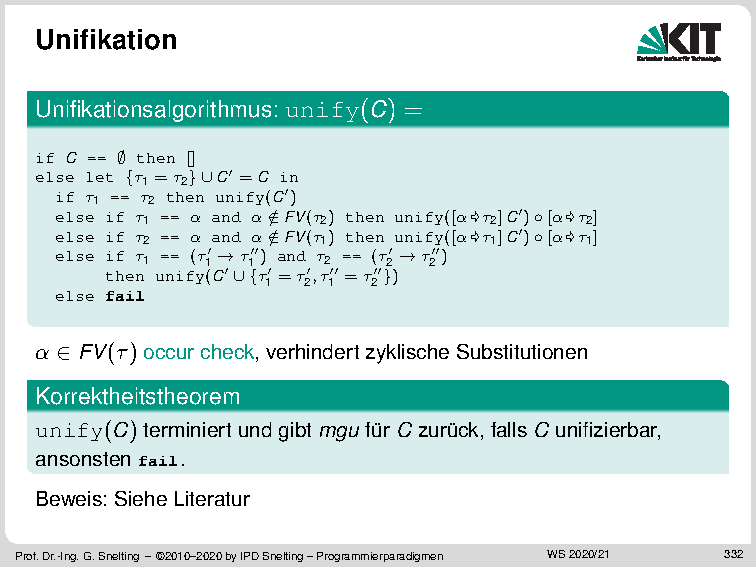
\includepdf{robinson2.pdf}
}

\begin{frame}{Unifikation für Typinferenz}
  \begin{itemize}
    \item Wir können den Robinson-Algorithmus 1:1 für die Typinferenz übernehmen.
    \item Statt Prolog-Termen verwenden wir Typterme:
    \begin{itemize}
      \item Konkrete Typen: int, string, char, etc. $\approx$ \pa{int}, \pa{string}, ...
      \item Typvariablen: $\alpha$, $\tau$ $\approx$ $A, X, ...$
      \item Funktionstypen: $\tau_1 \to \tau_2$ $\approx$ $\functor{f}{A, B}$
    \end{itemize}
    \item Wir könnten den Algorithmus noch erweitern um:
    \begin{itemize}
      \item Tupel, Listen, Dictionaries, etc.
      \item Machen wir aber nicht weil auch diese als Funktoren darstellbar sind $\leadsto$ Robinson für Prolog reicht
    \end{itemize}
  \end{itemize}
\end{frame}

\begin{frame}{Aufgabe: Unifikation für Typinferenz}
  \only<1>{
    \begin{align*}
      C_1 = \{ & \alpha_1 = \alpha_2 \to \alpha_3, \alpha_3 = \alpha_4 \to \alpha_5, \alpha_2 = \alpha_5 \} \\
      C_2 = \{ & \alpha_1 = \alpha_2 \to \alpha_3, \alpha_4 = \alpha_5 \to \alpha_3, \\
               & \alpha_2 = \alpha_4, \\
               & \alpha_5 = \alpha_6 \to \alpha_7, \alpha_6 = \alpha_7 \\
            \} &
    \end{align*}

    \begin{equation*}
      \sigma_1 = \texttt{unify}(C_1) = \unifier{\su{\alpha_1}{\alpha_5 \to \alpha_4 \to \alpha_5}, \su{\alpha_2}{\alpha_5}, \su{\alpha_3}{\alpha_4 \to \alpha_5}}
    \end{equation*}

    Der Typ von $\lam{x}{\lam{y}{x}}$ ist also $\sigma_1(\alpha_1) = \alpha_5 \to \alpha_4 \to \alpha_5$.

    \vfill
  }

  Findet den Typen von $\lam{f}{\app{f}{(\lam{x}{x})}}$!

  \only<2>{
    \begin{align*}
       & \sigma_2 = \texttt{unify}(C_2) \\
      =& \; \texttt{unify}(\{ \alpha_1 = \alpha_2 \to \alpha_3, ... \}) \\
      =& \; \texttt{unify}(\{ \alpha_4 = \alpha_5 \to \alpha_3, ... \}) \circ \unifier{\su{\alpha_1}{\alpha_2 \to \alpha_3}} \\
      =& \; \texttt{unify}(\{ \alpha_2 = \alpha_5 \to \alpha_3, ... \}) \circ \unifier{\su{\alpha_4}{\alpha_5 \to \alpha_3}} \circ \unifier{\su{\alpha_1}{\alpha_2 \to \alpha_3}} \\
      =& \; ... \\
      =& \; \unifier{
        \su{\alpha_1}{((\alpha_7 \to \alpha_7) \to \alpha_3) \to \alpha_3},
        ...
      }
    \end{align*}

    $\leadsto$ Der Typ von $\lam{f}{\app{f}{(\lam{x}{x})}}$ ist $((\alpha_7 \to \alpha_7) \to \alpha_3) \to \alpha_3$.
  }
\end{frame}

\subsection{\textsc{Let}-Polymorphismus}

\begin{frame}{\textsc{Let}-Polymorphismus: Motivation}
  \begin{equation*}
    \lam{f}{\app{f}{f}}
  \end{equation*}

  \begin{itemize}
    \item Diese Funktion verwendet $f$ auf zwei Arten:
    \begin{itemize}
      \item $\alpha \to \alpha$: Rechte Seite.
      \item $(\alpha \to \alpha) \to (\alpha \to \alpha)$: Linke Seite, nimmt $f$ als Argument und gibt es zurück.
    \end{itemize}
    \pause
    \item Problem: $\alpha \to \alpha$ und $(\alpha \to \alpha) \to (\alpha \to \alpha)$ sind nicht unifizierbar!
    \begin{itemize}
      \item \enquote{occurs check}: $\alpha$ darf sich nicht selbst einsetzen.
    \end{itemize}
  \item Idee: Bei jeder Verwendung eines polymorphen Typen erzeugen wir \emph{neue Typvariablen}, um diese Beschränkung zu umgehen.
  \end{itemize}
\end{frame}

\begin{frame}{Typschemata und Instanziierung}
  \only<1>{
    \begin{itemize}
      \item Idee: Bei jeder Verwendung eines polymorphen Typen erzeugen wir \emph{neue Typvariablen}, um diese Beschränkung zu umgehen.
      \item Ein \emph{Typschema} ist ein Typ, in dem manche Typvariablen allquantifiziert sind:
    \end{itemize}

    \begin{align*}
      \phi     & = \forall \alpha_1 . \; ... \; \forall \alpha_n . \tau \\
      \alpha_i & \in FV(\tau)
    \end{align*}

    \begin{itemize}
      \item \emph{Typschemata kommen bei uns immer nur in Kontexten vor!}
      \item Beispiele:
      \begin{itemize}
        \item $\forall \alpha . \alpha \to \alpha$
        \item $\forall \alpha . \alpha \to \beta \to \alpha$
      \end{itemize}
    \end{itemize}

  }

  \only<2>{
    \begin{itemize}
      \item Ein Typschema spannt eine Menge von Typen auf, mit denen es \emph{instanziiert} werden kann:
    \end{itemize}

    \begin{align*}
      \forall \alpha . \alpha \to \alpha & \succeq \text{int} \to \text{int} \\
      \forall \alpha . \alpha \to \alpha & \succeq \tau \to \tau \\
      \forall \alpha . \alpha \to \alpha & \not\succeq \tau \to \sigma \\
      \forall \alpha . \alpha \to \alpha & \not\succeq \tau \to \tau \to \tau \\
      \forall \alpha . \alpha \to \alpha & \succeq (\tau \to \tau) \to (\tau \to \tau)
    \end{align*}
  }
\end{frame}

\begin{frame}{\textsc{Let}-Polymorphismus}
  \only<1>{
    Um Typschemata bei der Inferenz zu verwenden, müssen wir zunächst die Regel für Variablen anpassen:

    \begin{mathpar}
      \inferrule{
        \Gamma(x) = \phi \\
        \phi \succeq_{\text{frische $\alpha_i$}} \tau
      }{
        \Gamma \vdash x : \alpha_j
      } \textsc{Var} \\
      \text{Constraint:} \; \{ \alpha_j = \tau \}
    \end{mathpar}

    \begin{itemize}
      \item $\succeq_\text{frische $\alpha_i$}$ instanziiert ein Typschema mit $\alpha_i$, die noch nicht im Baum vorkommen.
      \item Jetzt brauchen wir noch eine Möglichkeit, Typschemata zu erzeugen.
    \end{itemize}
  }

  \only<2>{
    Mit einen \textsc{Let}-Term wird ein Typschema eingeführt:

    \begin{mathpar}
      \inferrule{
        \Gamma \vdash t_1 : \alpha_i \\
        \Gamma' \vdash t_2 : \alpha_j
      }{ 
        \Gamma \vdash \texttt{let} \;\; x = t_1 \;\; \texttt{in} \;\; t_2 : \alpha_k
      } \textsc{Let}
    \end{mathpar}

    \pause

    \begin{align*}
      \sigma_{let} &= mgu(C_{let}) \\
           \Gamma' &= \sigma_{let}(\Gamma), x : ta(\sigma_{let}(\alpha_i), \sigma_{let}(\Gamma)) \\
          C'_{let} &= \{ \alpha_n = \sigma_{let}(\alpha_n) \mid \sigma_{let}(\alpha_n) \;\; \text{ist definiert} \}
    \end{align*}

    Constraints: $C'_{let} \cup C_{body} \cup \{ a_j = a_k \}$
  }
\end{frame}

\begin{frame}{Beispiel: \textsc{Let}-Polymorphismus}
    \scriptsize
    \begin{mathpar}
      \inferrule{
        \inferrule{
          ...
        }{
          \vdash \lam{x}{x} : \alpha_2
        } \textsc{Abs} \\
        \inferrule{
          \inferrule{
            \Gamma'(f) = \forall \alpha_5 . \alpha_5 \to \alpha_5 \\\\
            \succeq \alpha_8 \to \alpha_8
          }{
            \Gamma' \vdash f : \alpha_6
          } \textsc{Var} \\
          \inferrule{
            \Gamma'(f) = \forall \alpha_5 . \alpha_5 \to \alpha_5 \\\\
            \succeq \alpha_9 \to \alpha_9
          }{
            \Gamma' \vdash f : \alpha_7
          } \textsc{Var}
        }{
          \Gamma' \vdash \app{f}{f} : \alpha_3
        } \textsc{App}
      }{ 
        \vdash \texttt{let} \;\; f = \lam{x}{x} \;\; \texttt{in} \;\; \app{f}{f} : \alpha_1
      } \textsc{Let}
    \end{mathpar}

    \begin{align*}
           C_{let} &= \{ \alpha_2 = \alpha_4 \to \alpha_5, \alpha_4 \to \alpha_5 \} \\
      \sigma_{let} &= \unifier{\su{\alpha_2}{\alpha_5 \to \alpha_5}, \su{\alpha_4}{\alpha_5}} \\
      \Gamma'      &= x : \forall \alpha_5 . \alpha_5 \to \alpha_5 \\
          C'_{let} &= \{ \alpha_2 = \alpha_5 \to \alpha_5, \alpha_4 = \alpha_5 \} \\
          C_{body} &= \{ \alpha_6 = \alpha_7 \to \alpha_3, \alpha_6 = \alpha_8 \to \alpha_8, \alpha_7 = \alpha_9 \to \alpha_9 \} \\
                 C &= C'_{let} \cup C_{body} \cup \{ \alpha_3 = \alpha_1 \}
    \end{align*}
\end{frame}

\section{Ende}

\begin{frame}{Ende}
  Von heute mitnehmen:

  \begin{itemize}
    \item Robinson-Unifikation für Prolog-Terme und Lambda-Typen
    \item Typinferenz:
    \begin{itemize}
      \item Baum aufstellen
      \item Constraints aufsammeln
      \item mgu per Robinson berechnen
    \end{itemize}
  \end{itemize}

  Nächste Tuts:

  \begin{itemize}
    \item Compilerbau-Grundlagen
    \item Wir schreiben einen Compiler für Brainfuck: \texttt{++++++[>+++++++<-]>.}
  \end{itemize}
\end{frame}

\end{document}
